\documentclass[11pt,a4paper]{article}
\usepackage[margin=2.3cm]{geometry}
\usepackage[T1]{fontenc}
\usepackage{lmodern}
\usepackage{booktabs}
\usepackage{graphicx}
\usepackage{listings}
\usepackage{xcolor}
\usepackage[hidelinks]{hyperref}
\usepackage{url}
\urlstyle{tt}
\def\UrlBreaks{\do\/\do\_\do\=\do\(\do\)\do\*\do\,\do\.\do\-\do\:\do\+\do\|}

\lstset{
  basicstyle=\ttfamily\small,
  breaklines=true,
  frame=single,
  backgroundcolor=\color{black!4},
  columns=fullflexible,
  keepspaces=true
}
\newcommand{\file}[1]{\texttt{\path{#1}}}
\newcommand{\todo}[1]{\textcolor{red!70!black}{\textbf{TODO:} #1}}

\title{Coupled SOLPS--GOAT run: generating the GOAT inputs\\and checking the grid}
\author{}
\date{\today}

\begin{document}
\maketitle

%=========================================================================
\section{Working directories}
%=========================================================================
Two directories are used throughout this note:

\begin{center}
\begin{tabular}{@{}ll@{}}
\toprule
name & location \\
\midrule
\texttt{solps\_baserun} & \file{$SOLPSTOP/whateverrundir/baserun} \\
\texttt{goat\_run}      & \file{$GOATTOP/whateverrundir/} \\
\bottomrule
\end{tabular}
\end{center}

\noindent
\texttt{solps\_baserun} is the SOLPS base run, where the geometry is built in
DG and where the EFIT equilibrium lives. \texttt{goat\_run} is the GOAT run
directory, where GOAT is executed.
For example, for the TCV shot 87672:
\begin{lstlisting}[language=bash]
solps_baserun = $SOLPSTOP/runs/TCV/TCV87672/SILO_goatCoupled/baserun
goat_run      = $GOATTOP/runs/TCV/TCV87672/SILO_widegrid_equ2
\end{lstlisting}

%=========================================================================
\section{Procedure}
%=========================================================================

%-------------------------------------------------------------------------
\subsection{GOAT inputs}
%-------------------------------------------------------------------------
GOAT needs three inputs: \file{structure.dat}, \file{GOAToptions.dat} and the
magnetic equilibrium (\file{EQDSK_*.equ}, an \file{.equ} file in DG format).
Following the GOAT README, the vessel structures in \file{structure.dat}
should form a set of closed, nested, non-self-intersecting polygons, such that
the interior of the domain is well defined.

\subsubsection{\texorpdfstring{\texttt{structure.dat}}{structure.dat} from \texorpdfstring{\texttt{dg.dgo}}{dg.dgo}}

\paragraph{Prerequisite.}
The vessel and target specification is complete in DG and \file{dg.dgo} is
saved in \texttt{solps\_baserun}. The converter needs the sections
\texttt{p1}, \texttt{p2} and \texttt{fclbl}.

\paragraph{What the script does.}
The script is \file{scripts.local/dgo_to_structure.py}.
\begin{enumerate}
  \item It reads the segment end points $(X,Y[,Z])$ from the \texttt{p1} and
        \texttt{p2} sections and the integer labels from \texttt{fclbl}. All
        other sections of the \file{.dgo} file (\texttt{misselem},
        \texttt{jliin}, \dots) are ignored.
  \item It converts coordinates from mm to m and takes $X\to R$, $Y\to Z$.
  \item It groups segments by \texttt{fclbl}. Segments with label $\le 0$ are
        dropped; if there is no \texttt{fclbl} section every segment gets
        label~1.
  \item Within each label it chains segments into polylines, following the
        \texttt{p1}$\to$\texttt{p2} direction and joining end points that
        coincide within \texttt{--tol} (default $10^{-6}$\,m).
  \item It writes the Carre-format \file{structure.dat}:
        the first line is the number of structures, followed by
        \texttt{\$structures}; each structure is a block
        \texttt{Structure <label>} with a signed point count
        (negative: open chain; positive: closed loop, first point repeated at
        the end); the file ends with \texttt{\$end}.
  \item It prints whether all the pieces together form a single closed
        contour, and in which label order. This is the main check for a vessel.
\end{enumerate}

\paragraph{Usage.}
From \texttt{solps\_baserun}:
\begin{lstlisting}[language=bash]
python3 /pfs/work/g2etonel/solps-iter_3.2.1/scripts.local/dgo_to_structure.py \
    --in dg.dgo --out structure.dat [--tol 1e-6]
\end{lstlisting}
Defaults are \file{dg.dgo} and \file{structure.dat}. (The docstring of the
script refers to \file{scripts/}, but the file lives in \file{scripts.local/}.)

\paragraph{Checks.}
\begin{itemize}
  \item The script should print \texttt{Global contour closed: True}. For the
        \file{SILO_goatCoupled} \file{dg.dgo} it prints
        \texttt{Closed order (labels): [1, 7, 2, 6, 4, 5, 3]} (7 structures).
  \item If it prints \texttt{False}, there is a gap or a wrongly oriented
        segment in DG. Fix it in DG, or increase \texttt{--tol} if the gap is
        only rounding.
  \item The converter is best-effort: inspect the order and orientation of the
        structures if the topology is unusual.
  \item The structure labels matter later: \file{GOAToptions.dat} refers to
        structures by their number (target plates, refinement; see below).
\end{itemize}

\subsubsection{\texorpdfstring{\texttt{GOAToptions.dat}}{GOAToptions.dat}}

\file{GOAToptions.dat} holds all user options for GOAT. It is best to start
from an existing example (the GOAT README suggests copying one of
\file{$GOATTOP/Examples/*/GOAToptions.dat}). A complete working TCV example
(shot 87672, lower single null, \file{SILO_widegrid_equ2}) is reproduced in
Appendix~\ref{app:goatoptions}.

The options that are specific to the case, and must be reviewed for a new one,
are in particular:
\begin{itemize}
  \item the input file names: \texttt{goat.gridfilepath},
        \texttt{goat.magneticfieldfilepath} (the equilibrium file, read with
        \texttt{goat.mf.readmeth = 'equ'}), \texttt{goat.structurefilepath};
  \item \texttt{goat.data.RBtor}: here $1.2647534660\ldots =
        0.88\,\mathrm{m}\times 1.4372\,\mathrm{T}$, i.e.\ the \texttt{rtf} and
        \texttt{btf} values in the header of the equilibrium file;
  \item the target plates: \file{goat.vessel.TP}, \file{goat.vessel.TPind},
        \file{goat.vessel.solps_lower_divertor_inner_target} and
        \file{..._outer_target}. These are \emph{structure numbers}
        in \file{structure.dat} (here structures 1 and 2: inner and outer
        lower target);
  \item the outer and inner midplane positions \texttt{goat.data.OMPr/z} and
        \texttt{IMPr/z};
  \item the refinement and grid-density options (\texttt{gg.ref.*},
        \texttt{gg.radref.*}, \texttt{gg.vd.*}), including the structure
        IDs they refer to (\texttt{gg.ref.LB.structureIDs},
        \texttt{gg.ref.BL.structureID}).
\end{itemize}

\subsubsection{\texorpdfstring{\texttt{EQDSK\_*.equ}}{EQDSK\_*.equ} from the EFIT equilibrium with \texttt{e2d}}

\texttt{e2d} (\file{scripts/e2d}, \file{modules/DivGeo/equtrn/e2d}) is a thin
ksh wrapper around \texttt{ef2dg} that converts an EFIT equilibrium to the DG
format:
\begin{lstlisting}[language=bash]
e2d <EFIT-file> <DG-file>
# e.g.
e2d EQDSK_87672t1.2000_COCOS04x2 EQDSK_87672t1.2000_COCOS04x2.eq
\end{lstlisting}
The first argument is the input EFIT (g-eqdsk) file, the second the output
DG-format equilibrium. The script exits with a usage message if the input is
missing or unreadable.

\paragraph{Points to check.}
\begin{itemize}
  \item The extension is not prescribed: the existing TCV runs use
        \file{EQDSK_87672t1.2000_COCOS04x2.eq}, and whatever name is chosen
        must match \file{goat.magneticfieldfilepath} in
        \file{GOAToptions.dat}. (In SOLPS runs \file{dg.equ} is a symbolic
        link to this file.)
  \item The output header should contain the DG description of \texttt{jm},
        \texttt{km}, \texttt{r}, \texttt{z}, \texttt{psi}, \texttt{psib},
        \texttt{btf}, \texttt{rtf}, with \texttt{psi} as flux per radian
        [Wb/rad].
  \item The COCOS convention of the EFIT file matters: \texttt{e2d} does not
        convert it.
\end{itemize}

\subsubsection{Collecting the inputs}

\begin{enumerate}
  \item Finish the geometry in DG $\rightarrow$ \file{dg.dgo}.
  \item Run \file{dgo_to_structure.py} $\rightarrow$ \file{structure.dat};
        check that the contour is closed.
  \item Run \texttt{e2d} $\rightarrow$ equilibrium file.
  \item Prepare \file{GOAToptions.dat} (Appendix~\ref{app:goatoptions}).
  \item Put the three files in \texttt{goat\_run}:
\begin{lstlisting}[language=bash]
cp $SOLPSTOP/whateverrundir/baserun/structure.dat \
   $SOLPSTOP/whateverrundir/baserun/EQDSK_*.eq    $GOATTOP/whateverrundir/
# plus GOAToptions.dat edited for the case
\end{lstlisting}
\end{enumerate}

%-------------------------------------------------------------------------
\subsection{Running GOAT and checking the geometry}
%-------------------------------------------------------------------------
\paragraph{Environment.}
GOAT must be set up in a \emph{clean tcsh} terminal; the SOLPS setup file must
\emph{not} have been sourced in that shell, since it hampers compilation and
running of GOAT (GOAT README). From the top GOAT directory:
\begin{lstlisting}[language=bash]
tcsh
cd $GOATTOP         # i.e. the GOAT top directory
source setup.csh    # sets GOATTOP, PATH (goat.exe) and the pggoutput alias
\end{lstlisting}

\paragraph{Run GOAT.}
\begin{lstlisting}[language=bash]
cd $GOATTOP/whateverrundir
goat.exe            # or goat_debug.exe
\end{lstlisting}
GOAT reads \file{GOAToptions.dat} from the current directory. On success it
writes the grid \file{traduit.out.b2us} (the input for the SOLPS preprocessor
\texttt{b2ag}, together with \file{b2ag.dat}) and diagnostic data in
\file{./output}. Note that an existing \file{traduit.out.b2us} is
overwritten (\texttt{goat.writefilepath} in the TCV example).

\paragraph{Check the geometry with \texttt{pggoutput}.}
\texttt{pggoutput} is a tcsh alias, defined in \file{setup.csh}, for
\file{$GOATTOP/scripts/VisualizeGGOutput.py}. Run it from \texttt{goat\_run}:
\begin{lstlisting}[language=bash]
pggoutput                    # defaults: traduit.out.b2us, topomesh.dat, structure.dat
pggoutput <grid> <topomesh> <structure>   # non-standard names (optional arguments)
\end{lstlisting}
It reads the grid from the current directory and the diagnostics from
\file{./output}, and needs Python with Matplotlib, NumPy and Shapely. The
figures it produces include:
\begin{itemize}
  \item \emph{Topological mesh} (\file{output/topomesh.dat});
  \item \emph{Grid cells};
  \item \emph{Vessel structures} (from \file{structure.dat}), and the void
        polygons from \file{fort.78} if present;
  \item \emph{Face labels};
  \item \emph{Cell flux tube numbers} (cell regions);
  \item \emph{Face regions};
  \item the radial density function and the poloidal refinement lengths
        (\texttt{Lmin/Lmax}), and face intersections if present.
\end{itemize}

\paragraph{Topology check.}
In particular, check that the topology is correct. For the TCV lower single
null case:
\begin{itemize}
  \item the vessel structures plot shows the structures in the expected
        places and the target plates (structures 1 and 2 in the example)
        are the inner and outer lower divertor targets, as set in
        \texttt{goat.vessel.TP} and
        \texttt{goat.vessel.solps\_lower\_divertor\_*\_target};
  \item the topological mesh and the cell/flux-tube numbering show the
        expected regions: the lower X-point with the separatrix, the
        scrape-off layer, and the private-flux region below the X-point,
        with the inner and outer divertor legs ending on the two targets;
  \item the core region is removed (\texttt{gg.tm.removecoreregions = 1}),
        with the core boundary where expected (\texttt{gg.tm.addcoreboundaries});
  \item the face labels on the boundaries agree with the structures (labels
        are structure-based, \texttt{gg.labels.structurebased = 1}), in
        particular the target faces carry the target structure labels;
  \item there are no overlapping cells or face intersections and no
        unexpectedly narrow cells at the targets or X-point (\texttt{gg.vd.*}
        post-processing options);
  \item the grid does not leave unwanted gaps against the vessel (compare
        with the vessel structures figure).
\end{itemize}

Figure~\ref{fig:pgg} shows three of the plots of \texttt{pggoutput} for the
TCV case of Appendix~\ref{app:goatoptions}. Compare them with the checklist
above.

\begin{figure}[htbp]
  \centering
  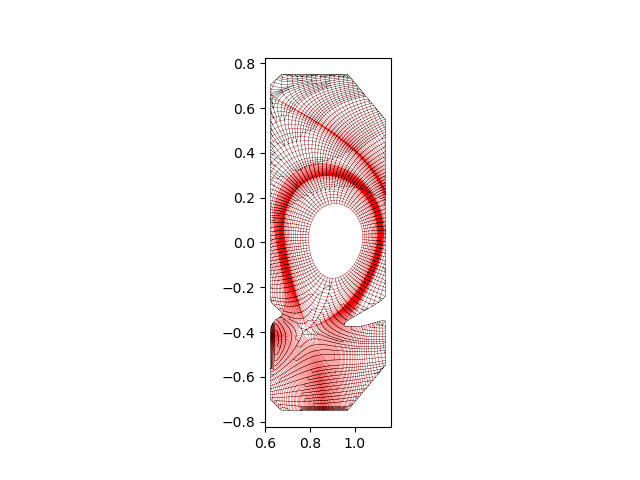
\includegraphics[height=8cm,trim=155bp 32bp 169bp 36bp,clip]{mesh_red.png}\hfill
  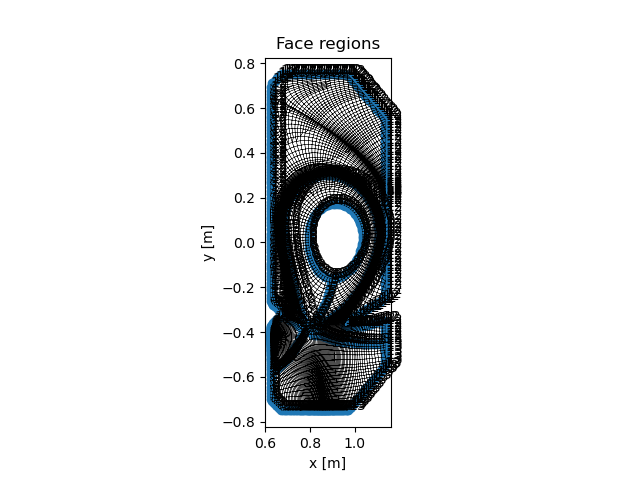
\includegraphics[height=8cm,trim=140bp 4bp 169bp 20bp,clip]{facelbl.png}\hfill
  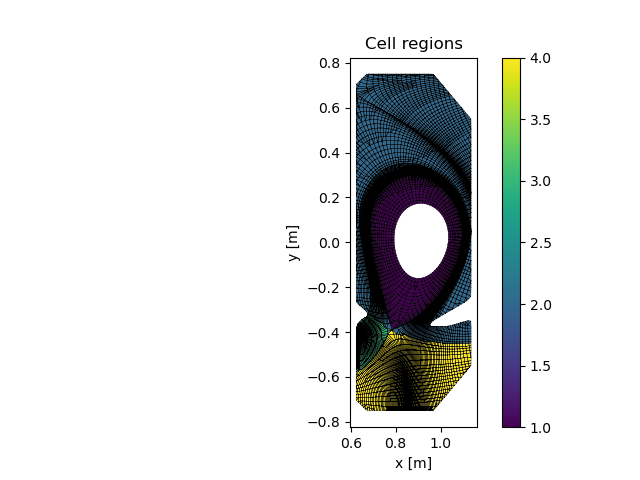
\includegraphics[height=8cm,trim=215bp 4bp 50bp 20bp,clip]{regions.png}
  \caption{Output of \texttt{pggoutput} for the TCV 87672 lower single null
  case. Left: grid cells. Centre: face regions (highlighted faces: vessel wall
  and inner boundary around the removed core region). Right: cell regions
  (flux tube regions), numbered as in the colour bar.}
  \label{fig:pgg}
\end{figure}

\todo{Describe the typical failure modes seen so far (wrong region numbering,
missing target faces, \dots).}

%=========================================================================
\appendix
\section{\texttt{GOAToptions.dat} for TCV}\label{app:goatoptions}
%=========================================================================
Taken from
\par\noindent\file{/pfs/work/g2etonel/goat_azito/runs/TCV/TCV87672/SILO_widegrid_equ2/GOAToptions.dat}\par
(TCV shot 87672, $t=1.2$\,s, lower single null).

\begin{lstlisting}
#=========================================================================#
#                                                                         #
#                       GENERAL GOAT OPTIONS                              #
#                                                                         #
#=========================================================================#
#-------------------------------------------------------------------------#
#                          MAIN OPTIONS                                   #
#-------------------------------------------------------------------------#
# General options
'goat.debug'                        '0'
'goat.meth'                         'GG'

# Input file locations 
'goat.gridfilepath'                 'traduit.out.b2us'
'goat.magneticfieldfilepath'        'EQDSK_87672t1.2000_COCOS04x2.eq'
'goat.structurefilepath'            'structure.dat'
'goat.GDinputfilepath'              'GOAToptions.dat'

# Output file locations 
'goat.writefilepath'                'traduit.out.b2us'  

# Output options 
'goat.write_final'                  '1'
'goat.write_traduitb2us'            '1'
'goat.write_b2agdat'                '1'
'goat.write_Xpointdata'             '0'
'goat.write_OMPdata'                '0'
'goat.write_topologicaldata'        '0'

# Switches to identify case
'goat.vesselmode'                   '1'
'goat.slab'                         '0'
'goat.artificial_slab'              '0'


#-------------------------------------------------------------------------#
#                          GRID OPTIONS                                   #
#-------------------------------------------------------------------------#
# Read method 
'goat.grid.readmeth'                'traduitb2us' 

# Grid type
'goat.grid.type'                    'plasma'

#-------------------------------------------------------------------------#
#                          MAGNETIC FIELD OPTIONS                         #
#-------------------------------------------------------------------------#
# Read method
'goat.mf.readmeth'                  'equ'

# Interpolation options
'goat.mf.interpC'                   '3'
'goat.mf.interpM'                   '6'
'goat.mf.interpmeth'                'uniformgrid'
'goat.mf.reinterpolate'             '0'
'goat.mf.resx'                      '200'
'goat.mf.resy'                      '200'

'goat.data.RBtor'                   '1.2647534660247'

#-------------------------------------------------------------------------#
#                          VESSEL STRUCTURE OPTIONS                       #
#-------------------------------------------------------------------------#
# Environment (including vessel etc) options 
# Vessel geometry & reading method
'goat.vessel.readmeth'              'read_structure'

# Refinement options for vessel
'goat.vessel.refinevessel'          '1'
'goat.vessel.maxvesseldist'         '1e-3'
'goat.vessel.minreffac'             '0'

# Target plate definition
'goat.vessel.TP'                    '[1, 2]'
'goat.vessel.TPind'                 '[1, 2]'

# SOLPS divertor targets (lower single null;)
# required by the new GOAT primary-strike guard).
'goat.vessel.solps_lower_divertor_inner_target'   '[1]'
'goat.vessel.solps_lower_divertor_outer_target'   '[2]'


# Structures to be excluded when constructing vessel (if empty, all are included)
'goat.vessel.exclude'               '[]'

# Vessel field description (similar to magnetic field interpolant, 
# but for vessel - only used for vessel distance penalty, and if shape
# method is the same, also used for boundary constraints)
'goat.vessel.shapemeth'             'closedpolygon_exact'
'goat.vessel.resx'                  '100'
'goat.vessel.resy'                  '100'
'goat.vessel.offsetfracx'           '0.1'
'goat.vessel.offsetfracy'           '0.1'
'goat.vessel.interpC'               '3'
'goat.vessel.interpM'               '6'

#-------------------------------------------------------------------------#
#                          ADDITIONAL DATA                                #
#-------------------------------------------------------------------------#
# OMP and IMP
'goat.data.OMPr'                '[0.95 1.3]'
'goat.data.OMPz'                '[0 0]'
'goat.data.IMPr'                '[0.6 0.75]'
'goat.data.IMPz'                '[0 0]'

#=========================================================================#
#                                                                         #
#                         GRID GENERATION                                 #
#                                                                         #
#=========================================================================#
# Grid and magnetic field options are set through the standard grid 
# deformation options thereof. Here, only grid generation specific options
# are set. 
# General options
'gg.verbosity'                          '1'
'gg.vertexconstructionmethod'           'orthogonal'
'gg.TMcellgriddingorder'                'sequential'
'gg.cellconstructionmethod'             'quads_triangles'
'gg.ref.readexistingrefdata'            '0'
'gg.labels.structurebased'              '1'
'gg.dogriddiagnostics'                  '1'

#-------------------------------------------------------------------------#
#                         TOPOLOGICAL MESH OPTIONS                        #
#-------------------------------------------------------------------------#

# Read exising file? 
'gg.tm.readexistingTM'          '0'
'gg.tm.TMfilepath'              './output/topomesh.dat'

# Magnetic field: tracing & resolution (description is determined by GD options)
'gg.tm.field.resx'              '100'
'gg.tm.field.resy'              '100'
'gg.tm.field.donewton'          '1'
'gg.tm.fieldtol'                '1e-8'

# Tangency point tangency point treatment 
'gg.tm.dotpvesselbased'         '1' # best used in combination with vessel refinement

# Vessel contour tracing (vessel description is determined by GD options)
'gg.tm.vessel.resx'             '400'
'gg.tm.vessel.resy'             '400'
'gg.tm.vessel.donewton'         '0'

'gg.tm.contour.npmin'           '10'
'gg.tm.contour.npmax'           '10000'
'gg.tm.contour.dl'              '0.0075'

# Core boundary and region treatment
'gg.tm.doadaptations'           '1'
'gg.tm.addcoreboundaries'       '1'
'gg.tm.addPFboundaries'         '0'
'gg.tm.cbnd.frac'               '0.6'
'gg.tm.PFbnd.frac'              '0.1'
'gg.tm.removecoreregions'       '1'
'gg.tm.removewidegridregions'   '0'
'gg.tm.mergetangencypointtubes' '1'
'gg.tm.dpsimintangencypointtubes' '0.0'
'gg.tm.lradmintangencypointtubes' '2.0e-3'

'gg.tm.alignvesselparts'        '0'
'gg.tm.avpminangle'             '2.5'
'gg.tm.avprefinevessel'         '1'
'gg.tm.avpmaxvesseldist'        '2.0e-3'
'gg.tm.avpminreffac'            '10'
'gg.tm.mergeavptubes'           '0'
'gg.tm.mergetubes'              '1'
'gg.tm.mergetubes.meth'         'extensive'
'gg.tm.lradmintubes'            '1e-3'
'gg.tm.dpsimintubes'            '0.0'
'gg.tm.mergetubes.allowseparatrix'     '0'

#-------------------------------------------------------------------------#
#                         VERTEX DISTRIBUTION OPTIONS                     #
#-------------------------------------------------------------------------#


# adaptations
'gg.adap.extendtptubes'                 '1'
'gg.adap.extendvesseltubes'             '1'
'gg.adap.evt.maxvessellength'           '0.01'


# Refinement options
'gg.ref.meth'                           'lengthbased'
#'gg.ref.meth'                           'no'
'gg.ref.LB.doxp'                        '1'
'gg.ref.LB.dovessel'                    '1'
'gg.ref.LB.Lmininf'                     '0.005'
'gg.ref.LB.Lmaxinf'                     '0.02'
'gg.ref.LB.structureIDs'                '[1]'
'gg.ref.LB.Lminstructure'               '[0.01, 0.01]'
'gg.ref.LB.Lmaxstructure'               '[0.025, 0.025]'
'gg.ref.LB.decaylengthstructure'        '[0.25, 0.25]'
'gg.ref.LB.Lminxp'                      '0.01'
'gg.ref.LB.Lmaxxp'                      '0.05'
'gg.ref.LB.decaylengthxp'               '0.2'

# Refinement options
'gg.radref.meth'                           'lengthbased'
#'gg.radref.meth'                           'no'
'gg.radref.LB.lengthtype'                   'radial'
'gg.radref.LB.dosp'                        '1'

# Options for psi length type 
#'gg.radref.LB.Lmininf'                     '0.1'
#'gg.radref.LB.Lmaxinf'                     '0.5'
#'gg.radref.LB.Lminsp'                      '0.05'
#'gg.radref.LB.Lmaxsp'                      '0.12'
#'gg.radref.LB.decaylengthsp'               '0.5'

# Options for (radial) length type 
'gg.radref.LB.Lmininf'                     '0.01'
'gg.radref.LB.Lmaxinf'                     '0.05'
'gg.radref.LB.Lminsp'                      '0.0005'
'gg.radref.LB.Lmaxsp'                      '0.01'
'gg.radref.LB.decaylengthsp'               '0.3'


# Boundary layer options (only for length based refinement for now)
'gg.ref.BL.dotarget'                  '0'
'gg.ref.BL.nctarget'                  '7'
'gg.ref.BL.dltarget'                  '[0.002, 0.003, 0.004, 0.006, 0.008, 0.012, 0.016]'
'gg.ref.BL.dovessel'                  '0'
'gg.ref.BL.ncvessel'                  '7'
'gg.ref.BL.dlvessel'                  '[0.002, 0.003, 0.004, 0.006, 0.008, 0.012, 0.016]'
'gg.ref.BL.dllengthbased'             '1'

# 'Boundary' layer options for radial direction
'gg.radref.BL.dosp'                '0'
'gg.radref.BL.ncsp'                '6'
'gg.radref.BL.dlsp'                '[0.0010, 0.0015, 0.002, 0.003, 0.0045, 0.0067]'
'gg.radref.BL.dllengthbased'       '0'


'gg.ref.BL.dostructure'               '1'
'gg.ref.BL.structureID'               '[1, 2]'
'gg.ref.BL.ncstructure'               '4'
'gg.ref.BL.dlstructure'               '[0.003, 0.004, 0.005, 0.006]'

# Post-processing options
'gg.vd.removefluxsurfaces'              '1' # Remove too narrow flux surfaces
'gg.vd.removenarrowboundarytriangles'   '1' # Remove too narrow triangles at boundary and replace by cut cells

# Contour resolution 
'gg.vd.contouring.resx'         '400'
'gg.vd.contouring.resy'         '400'
'gg.vd.contouring.coarsen'      '1'

# Orthogonal line tracer options (only if orthogonal based GG is used)
'gg.vd.orthlinetracing.step'    '5' # relative step size (larger = less accurate but faster)
'gg.vd.orthlinetracing.nsteps'  '500' # maximal number of steps to take 

# Distribution of flux surfaces (radial)
'gg.vd.rd.type'                         'densitybased'

# Distribution of vertices on flux surfaces (poloidal)
'gg.vd.pd.type'                         'uniform'

# Options for uniform distribution
'gg.vd.pd.distribution.facelength'      '0.012'

'gg.vd.rd.distribution.fieldwidth'      '8e0'

# Options for density based distribution
'gg.vd.pd.distribution.plftype'            'target'
'gg.vd.pd.distribution.decaylengthplf'     '1.00'
'gg.vd.pd.distribution.densityatvessel' '100'
'gg.vd.pd.distribution.densityatinf'    '10'

# Options for density based distribution, radial
'gg.vd.rd.distribution.doxp'            '1'
'gg.vd.rd.distribution.decaylengthxp'   '0.02'
'gg.vd.rd.distribution.densityatxp'     '100'
'gg.vd.rd.distribution.densityatinf'    '50'
'gg.vd.rd.distribution.densityatsp'     '400'
'gg.vd.rd.distribution.decaylengthsp'   '0.1'

#'gg.vd.rd.distribution.points.x'        '[0.92, 0.92]'
#'gg.vd.rd.distribution.points.y'        '[-0.75, 0.75]'
#'gg.vd.rd.distribution.points.val'      '[100, 100]'
#'gg.vd.rd.distribution.points.d'        '[0.1, 0.1]'

# Options for remove narrow boundary triangles
'gg.vd.rnbt.mark.criterion'             'angle'
'gg.vd.rnbt.mark.minangle'              '5'
\end{lstlisting}

\end{document}
